
\subsection{Osvětlovací modely}
\subsection*{Druhy osvětlení}
Výpočet osvětlení, záleží na druhu osvětlení a optických vlastnostech těles.
Existují 3 druhy osvětlení:
\begin{itemize}
 	\item \textbf{Ambientní}  - fiktivní, všudypřítomné rozptýlené (dopadá na těleso rovnoměrně ze všech směrů)
 	\item \textbf{Difúzní} – matný odraz (intenzita, která se odráží od matného materiálu do všech směrů)
 	\item \textbf{Spekulární}  - odlesk (odrazivá složka – podle zákonů lomu)
\end{itemize}
\subsection*{Phongův osvětlovací model} % https://www.youtube.com/watch?v=L4oAQL_Mv5w
\begin{itemize}
	\item $I = I_a + I_d + I_s$ 
	\item Phongův osvětlovací model je empirický (na fyzice nezaložený) osvětlovací model pro výpočet osvětlení povrchu nějakého objektu.
	\item Ačkoliv tento model není fyzikálně zcela přesný, výsledky, které podává, jsou natolik zdařilé, že se Phongův model v počítačové grafice široce využívá již několik desítek let, zejména pak pro svou rychlost našel uplatnění v real-time grafice.
	\item Jeho nevýhodou je, že nedokáže simulovat některé optické jevy globálního osvětlení, jako např. Kaustiky (Kaustika je obálka světelných paprsků odražených nebo zlomených nějakou zakřivenou plochou nebo předmětem).
%	\item Vytváří na povrchu odlesky Výpočet je:
%	\begin{equation*} 
%			\begin{array}{c}
%				I_p = k_ai_a + \sum\limits_{m \in lights} (k_d(\vec{L_m} \cdot \vec{N})i_{m,d} + k_s(\vec{R_m} \cdot \vec{V})^\alpha i_{m,s}). \\
%			\end{array}
%			\end{equation*}
%
%		\begin{itemize}
%			\item kde: \textbf{a} -- ambientní, \textbf{d} -- difůzní, \textbf{s} -- spekulátní,
%			\item 	$lights$ -- je soubor všech světelných zdrojů,
%			\item 	$k$ -- parametry materiálu,
%			\item 	$i$ -- složka světla (intenzita),
%			\item 	$\alpha$ -- shininess -- udává ostrost spekulárního odrazu (velikost specular highlightu),
%			\item 	$L$ -- směr ke světlu,
%			\item 	$N$ -- normála v daném bodě,
%			\item 	$R$ -- směr dokonale odrazené svěla v daném bodě,
%			\item 	$V$ -- směr z bodu k pozorovateli (kameře).
%			\item Směr odraženého paprsku určuje vztah $\vec{R_m} = 2(\vec{L_m} \cdot \vec{N})\vec{N} - \vec{L_m}$.
%		\end{itemize}
		\begin{figure}[H]
		\centering
		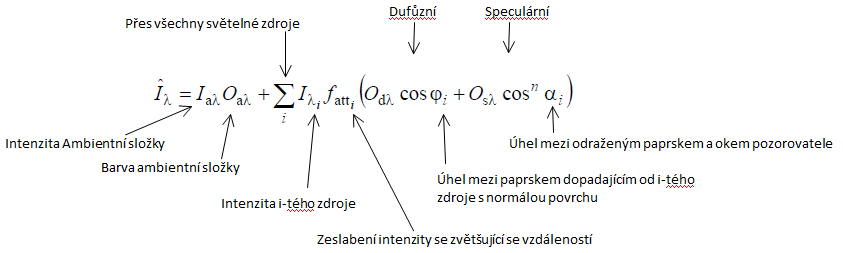
\includegraphics[width=1\textwidth]{assets/1_phong_model}
		\end{figure}
		 \subsubsection*{Zeslabení intenzity i--tého světelného zdroje}
		 \item kde $\mathbf{c_0,c_1,c_2}$ jsou konstanty popisující úbytek intenzity světla a $\mathbf{d_i}$ je vzdálenost. \\
		 $f_{att_i} = min \{\frac{1}{c_0+c_1d_i + c_2d_i^2}, 1\}$
		 \subsubsection*{Úhel mezi paprskem a normálou}
		 \item Kde $n$ je vektor normály plochy, $I_i$ je vektor směřující od místa, kde osvětlení počítám k $i$--tému světelnému zdroji. \\
		 $\cos{\varphi_i} = n \cdot l_i$
		 \begin{figure}[H]
		\centering
		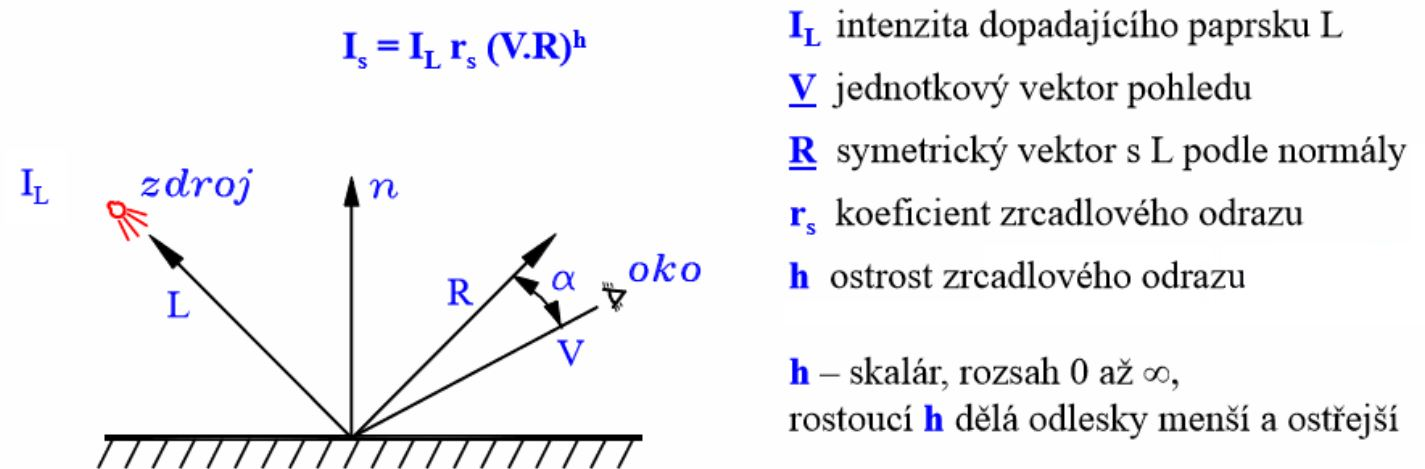
\includegraphics[width=1\textwidth]{assets/1_phong_zrcadlo}
		\end{figure}
\end{itemize}

\subsection*{Blinn-Phong osvětlovací model}
\begin{itemize}
	\item Výchozí osvětlovací model pro standardní zobrazovací řetězec v OpenGL/DirectX. Zavádí tzv. half vector.
	\item $ H = \frac{L + V}{| L + V |}$
	\item Místo $R \cdot V$  pak použijeme při výpočtu $N \cdot H$.
	\item Blinn-Phong \textbf{je pomalejší} než původní Phong, protože při výpočtu half vectoru je nutné provést odmocninu (při normalizaci).
	\item Jelikož je odmocnina \textbf{hardwarově implementovaná}, rozdíl je zanedbatelný.
	\item Je však \textbf{rychlejší}, když se pozorovatel a světlo předpokládá v nekonečnu -- směrová světla.
	\item V tom případě je half vector \textbf{nezávislý na poloze a zakřivení povrchu}, stačí jej vypočítat pouze jednou pro každé světlo.
\end{itemize}

\subsection{Systémy barev v PG}
\textbf{Barevný prostor}:
\begin{itemize}
	\item Základem barevného prostoru je \textbf{barevný model}, který nám dává abstraktní matematický popis, jak lze barvy vyjádřit pomocí n-tic čísel, nejčastěji trojic. 
	\item Mezi nejznámější barevné modely v dnešní době patří \textbf{RGB model}. 
	\item Model RGB pracuje se třemi základními barvami: \textbf{červenou, zelenou} a \textbf{modrou}, z nichž se odvíjí i jeho název. 
	\item Tyto barvy byly zvoleny na základně toho, jak \textbf{čípky v lidském oku} vnímají jednotlivé záření. 
	\item Zároveň je RGB \textbf{aditivní barevný model}, což znamená, že se jednotlivé barevné složky \textbf{míchají} a výsledkem jsou další barevné odstíny, případně vyšší intenzita barvy
	\item Když k tomuto modelu definujeme, jak mají být tyto n-tice interpretovány, dostáváme barevný prostor. 
	\item Barevný prostor je tedy \textbf{definován rozsahem barev}, které dokáže zobrazit. 
	\item Tomuto rozsahu se také říká \textbf{gamut}. Ten se zpravidla zobrazuje jako oblast v CIE 1931 chromatickém diagramu 
\end{itemize}
\begin{figure}[H]
\centering
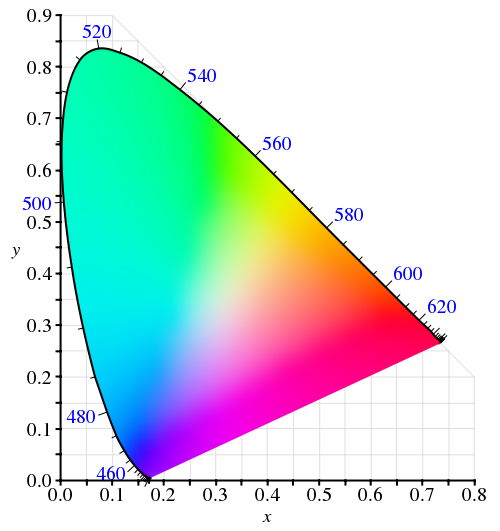
\includegraphics[width=0.3\textwidth]{assets/1_rgb_gamut}
\end{figure}
\subsubsection{RGB}
\begin{itemize}
	\item Nejrozšířenější barevný prostor postavený na RGB barevném modelu je \textbf{sRGB} - standardní RGB. 
	\item Jeho určení je pro zobrazování \textbf{na monitorech} nebo \textbf{kódování barev} na internetu. 
	\item Pro všechny tři barevné složky má definovány barvy v \textbf{chromatickém diagramu}, které vymezují jeho gamut. 
	\item Každá barva, kterou tento prostor zobrazuje, je dána zastoupením jednotlivých barevných složek, buďto relativně (hodnoty jsou v rozmezí 0 - 1) nebo absolutně (konkrétní \uv{bitové} hodnoty, zpravidla 0 - 255).
	\item RGB je možné zobrazit jako krychli.
	\item Často se přidává \textbf{Alpha kanál} pro průhlednost - \textbf{RGBA}.
	\begin{figure}[H]
	\centering
	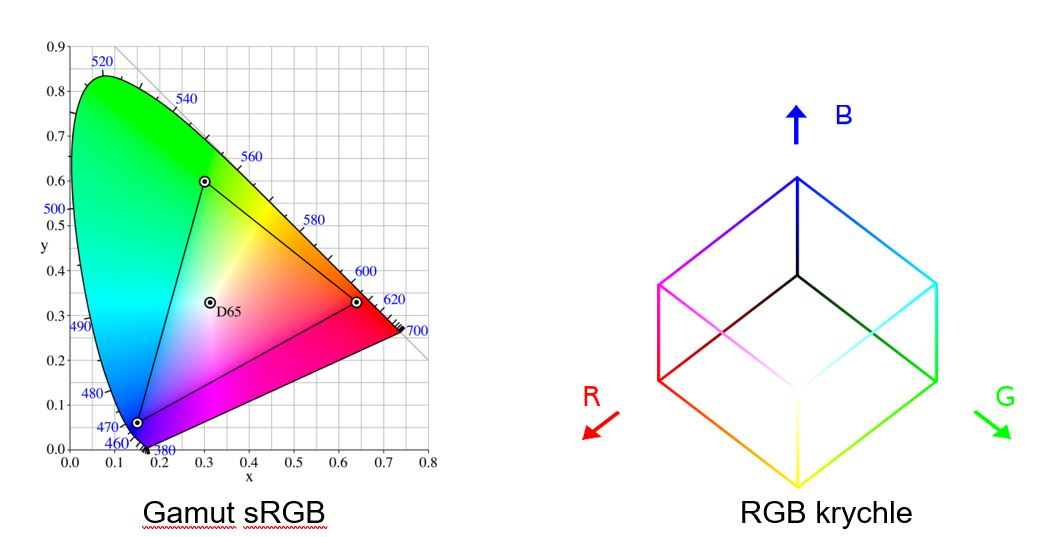
\includegraphics[width=0.6\textwidth]{assets/1_rgb_gamut_krychle}
	\end{figure}
\end{itemize}

\subsubsection{HSV a HSL}
\begin{itemize}
	\item \textbf{Hue, Saturation, Value/Lightness} - barevný model, který nejvíce odpovídá lidskému vnímání barev.
	\item Barvy popisuje pomocí 3 hodnot, které však samy barvy nereprezentují:
	\begin{itemize}
		\item \textbf{Hue} - \textbf{barevný tón}, převládající. Neboli odstín - barva \textbf{odražená} nebo \textbf{procházející} objektem. Měří se jako poloha na standardním barevném kole (\ang{0} až \ang{360}). Obecně se odstín označuje názvem barvy. \ang{0} - červená, \ang{120} - zelená, \ang{240} - modrá.
		\item \textbf{Saturation} - \textbf{sytost} barvy, příměs jiné barvy. Někdy též chroma, síla nebo čistota barvy, představuje množství šedi v poměru k odstínu, měří se v procentech od 0\% (šedá) do 100\% (plně sytá barva). Na barevném kole vzrůstá sytost od středu k okrajům.
		\item \textbf{Value} - \textbf{hodnota jasu}, množství bílého světla. Relativní světlost nebo tmavost barvy. Jas vyjadřuje \textbf{kolik světla barva odráží}, dalo by se také říct přidávání černé do základní barvy.
	\end{itemize}
	\item Nejčastěji se tato reprezentace (popř. \textbf{HSL}) používají v grafických nástrojích jako komponenty pro výběr barvy, protože je mnohem intuitivnější než RGB. 
	\item Vyberu si odstín, jak má být sytý a jasný a hotovo. Není třeba řešit jak smíchat 3 barevné složky, abych dostal to co chci.
	\begin{figure}[H]
	\centering
	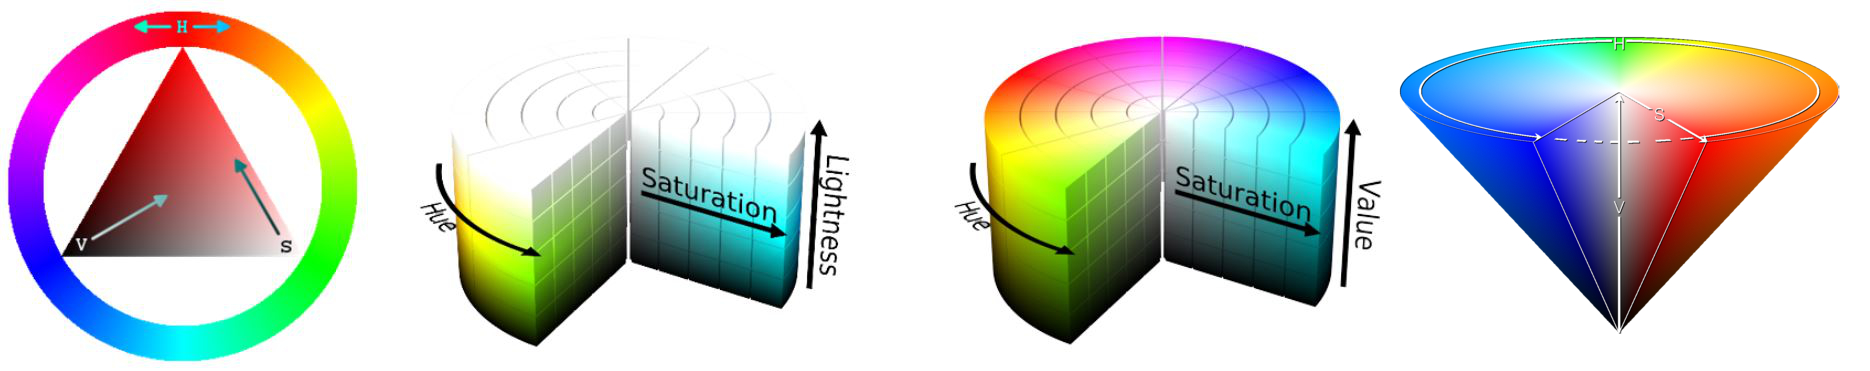
\includegraphics[width=0.6\textwidth]{assets/1_hsv_hsl}
	\end{figure}
\end{itemize}

\subsubsection{CMY a CMYK}
\begin{itemize}
	\item Substraktivní barevné systémy, \textbf{C}yan, \textbf{M}agenta, \textbf{Y}ellow a \textbf{K}ey (Blac\textbf{K}). 
	\item Barvy se \textbf{odečítají od bílé}.
	\item Používají se \textbf{pro tisk}.
	\item Černá se přidala, protože smíchání CMY nedává plně černou barvu, navíc je černý inkoust levnější než barevné.
	\item Nevýhodou je, že \textbf{nedokáže správně zobrazit} sytě červenou, zelenou a modrou.
	\item Při tisku to však není poznat.
	\item Před tiskem se RGB obraz převádí do CMYK.
	\item To provádí buďto ovladač tiskárny nebo RIP (Raster Image Processor - u profi tiskáren).
	\item RGB se používá pro aktivní zdroje světla, CMYK jsou pasivní (světlo pouze odrážejí), proto nedokáží udělat tak jasné odstíny.
\end{itemize}
	\begin{figure}[H]
	\centering
	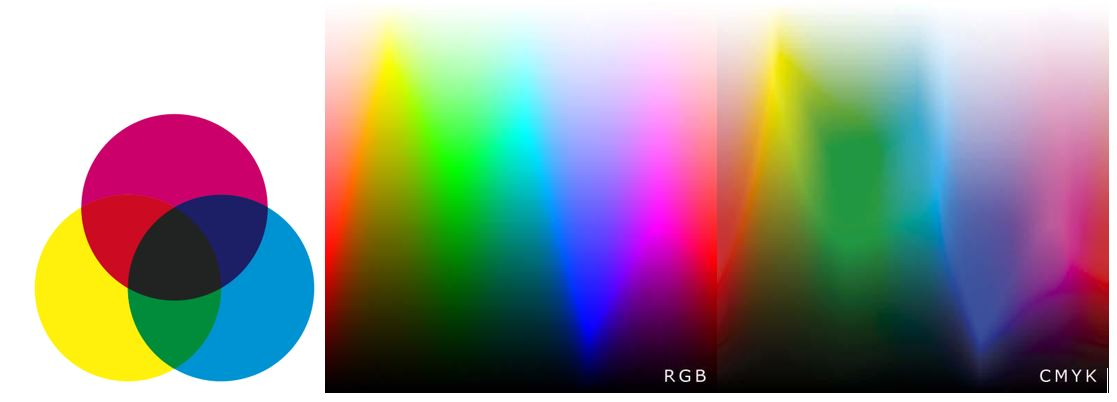
\includegraphics[width=0.6\textwidth]{assets/1_cmyk}
	\end{figure}